\documentclass[11pt]{article}

\usepackage{color}
\usepackage{caption}
\usepackage{amsmath}
\usepackage{amsthm}
\usepackage{amsfonts} 
\usepackage{amssymb}
\usepackage{multirow}
\usepackage[pdftex]{graphicx}
\usepackage{epsfig}
\usepackage{latexsym}
\usepackage{enumerate}
\usepackage{tabularx}
\usepackage{booktabs}
\usepackage{fullpage}
\usepackage{algorithm}
\usepackage{centernot}
\usepackage[noend]{algpseudocode}
\usepackage{setspace}
\usepackage{indentfirst}

\newtheorem{thm}{Theorem}
\newtheorem{problem}[thm]{Problem}
\newenvironment{claim}[1]{\par\noindent\textit{Claim:}\space#1}{}

\newcommand{\R}{\mathbb{R} }
\newcommand{\Q}{\mathbb{Q} }
\newcommand{\Z}{\mathbb{Z} }
\newcommand{\N}{\mathbb{N} }
\newcommand{\C}{\mathbb{C} }
\newcommand{\Prob}[1]{ \mathbb{P} \left[ #1 \right] }
\newcommand{\Given}{\middle|}
\newcommand{\overbar}[1]{\mkern 1.5mu\overline{\mkern-1.5mu#1\mkern-1.5mu}\mkern 1.5mu}

\begin{document}

\title{Visualizing Hillary Clinton's Emails}

\author{
  Yihe Chen \\
  \texttt{yc3076}
  \and 
  Palmer Lao \\
  \texttt{pol2105}
  \and
  Daitong Li \\
  \texttt{dl2991}
  \and
  Ziyue Shuai \\
  \texttt{zs2285}
  \and
  Eric Zhang \\ 
  \texttt{ez2232}
}

\date{\today}
\maketitle
\doublespacing


\section{Introduction}
In light of the recent U.S. presidential election race between candidates Donald Trump and Hillary Clinton, there have been large amounts of interest in the controversy involving Hillary's use of personal email accounts on non-government servers during her previous career as Secretary of State. 
After a number of Freedom of Information lawsuits were filed against the Department of State, the Department of State released on August 31, 2015 nearly 7,000 pages of Clinton's heavily redacted communications in PDF form.

Subsequent to this release, the data science competition website Kaggle released a sanitized version of the extracted content of the emails for public use and analysis. 
Our group was interested in analyzing and exploring this data given its connection to current events at the time.

\section{Objectives}
Our main objective with this project was to reduce the immense dimensionality and volume of the data so that the resulting output could be more easily digested by a data analyst or other interested party. We wanted to find patterns in the data that might be of interest, such as communities of receiving or sending parties that shared certain commonalities. 

We tried to discover such patterns through the application of three methods: Social Network Analysis (SNA), TextRank, and Cluster Analysis.

However, rather than simply report on the results of such analysis, we believed that a more effective way to communicate results and allow for the generation of new insights would be to create an interactive visualization that would empower the user to both view our findings and explore the simplified data at will.


\section{Data Source}
Some 7,000 pages of Clinton's emails were released by the State Department in PDF format.
Kaggle then scraped the text from these PDFs and hosted them as CSVs and SQL databases on the Kaggle Kernels platform.
The dataset contains nearly 8,000 emails sent within Clinton's inner circle from December 2010 to September 2012.

\begin{figure}[h]
  \centering
  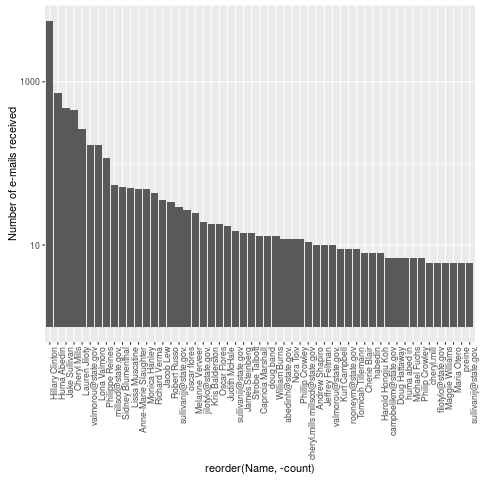
\includegraphics[scale=0.8]{palmer/graphics/num_recvd_histogram}
  \caption{Histogram of how many emails some person has received}
  \label{fig:n_recv_hist}
\end{figure}

\begin{figure}[h]
  \centering
  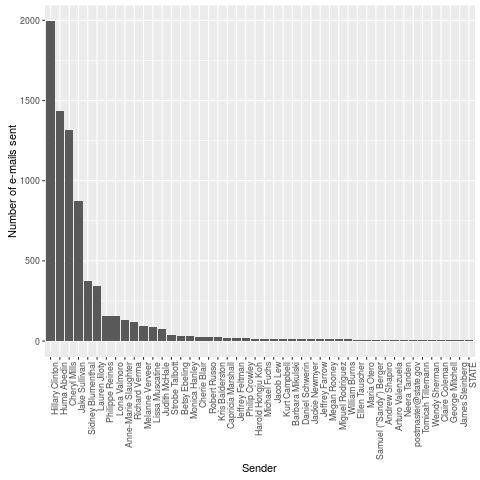
\includegraphics[scale=0.8]{palmer/graphics/num_sent_histogram}
  \caption{Histogram of how many emails some person has sent}
  \label{fig:n_sent_hist}
\end{figure}

Unsurprisingly, the email dataset seems to be Hillary-centric.
In addition, the histogram of emails received seems to be much more highly dispersed than the histogram of emails sent, which may suggest that many emails are sent to multiple people.



\section{Methodology}

\subsection{An Overview of our Summarization Procedure for one Document}
Because our end goal is to create a visual dashboard for our users, we have to be careful about our bookkeeping while we slice and dice our text data. 
A brief overview of our procedure from end-to-end for one e-mail is as follows:
\begin{enumerate}
\item Split the e-mail into sentences
\item Clean each sentence
\item Represent each sentence as a bag-of-words
\item Run TextRank to get a ranking of the bags-of-words
\item Return the top $k$ sentences from the original e-mail associated with the top $k$ ranking bags-of-words
\end{enumerate}

Of particular importance to our implementation is keeping track of how the bags-of-words are associated with the original sentences from the e-mail, as the bags-of-words are not nearly as informative to the user.

\subsection{The TextRank Algorithm}
We treat each e-mail as a self-contained document and attempt to summarize each document using TextRank \cite{textrank}, which is a derivative of PageRank \cite{pagerank} adapted to units of text instead of web pages.

The PageRank algorithm is a way of ranking web pages based on the way that they link to each other.
The algorithm is based on a random walk model of the typical internet user.
We assume the user starts on some arbitrary web page and then either randomly clicks links on the current page or with some re-seeding probability, $d$, navigates to another random web page that was not necessarily linked to from the current one.
The process of such a user's browsing history is clearly Markovian under this assumption.
The addition of the re-seeding probability makes this Markov process irreducible and aperiodic, or equivalently, ergodic \cite{intro-prob-models-ross}. 
Ergodicity allows us to conclude that there exists a so-called stationary distribution over the set of all web pages.
Moreover, this stationary distribution is unique and is the limit of a certain quantity.

The stationary distribution of an ergodic Markov chain has many interpretations.
One is that the distribution assigns probability mass to each state, where this mass is equivalent to the probability that the Markov process is observed in some state after the chain has mixed or lost its dependence on its initial position.
The other is the ``time-average'' interpretation: the average proportion of time-steps a process will spend in some state tends to this state's mass in the stationary distribution.

Web pages that are assigned a large probability mass are thought to be relatively important in the sense that a random web surfer is more likely to visit it.
One can sort the pages by the amount of mass assigned to them by the stationary distribution to get a ranking of pages by this notion of importance.

To turn this idea into something that can summarize text, we need to decide on two things.
The first is the notion of an item to rank, or in our case, a unit of text.
The second is the notion of how all items pairwise indicate each other's importance.

A typical choice of unit of text is either sentences or phrases.
We choose to rank sentences for the sake of simplicity.

For text, we might imagine that a sentence that is highly similar to many of the other sentences is important in the sense that it may mix the contents of the most sentences to provide an insightful summary of the entire document.
Naturally, we might choose to define the transition matrix of the Markov chain over sentences by the similarity between sentences, which now reduces our problem to figuring out a measure of pairwise similarity between sentences.

A naive view of sentences is to think of them as sets or multisets of words.
An easy measure of similarity over sets $S_1$, $S_2$ is the Jaccard similarity:
\begin{equation*}
  J(S_1, S_2) \triangleq \frac{|S_1 \cap S_2|}{|S_1 \cup S_2|}
\end{equation*}
which can easily be extended to multisets \cite{wiki:Multiset}.

We opt to use the recommendation of the original TextRank paper \cite{textrank}:
\begin{equation*}
  \text{Similarity}(S_1, S_2) \triangleq \frac{ | \{ w_k | w_k \in S_1 \& w_k \in S_2 \} |}{\log(|S_1|) + \log(|S_2|)}
\end{equation*}

although there are many other variations that we did not have the chance to evaluate \cite{textrank-sim-var}.

To actually compute the TextRank of a document represented as a collection of bags-of-words, we perform the following procedure:
\begin{enumerate}
\item For each pair of sentences $S_i$ and $S_j$, compute their similarity $\text{Similarity}(S_i, S_j)$ and store it in a matrix as entry $\tilde{M}_{ij}$.
\item Normalize $\tilde{M}$ to get a transition matrix $M$, representing a Markov chain over sentences.
\item Starting with an initial guess of the stationary distribution $R_0$, iteratively compute 
  \[
    R_{t+1} = dMR_t + \frac{1-d}{N} \mathbf{1},
  \]
where $d$ is the re-seeding probability, $N$ is the number of sentences, and $\mathbf{1}$ is a column vector of ones.
\item After enough iterations, $R_t$ will have nearly converged to the true stationary distribution of our damped Markov chain. The rankings of the probabilities in $R_t$ can be regarded as the TextRank of our document.
\end{enumerate}

Running an entirely analogous algorithm on the entirety of the web (a graph consisting of about 322 million edges) took the Sergey Brin and Larry Page, the authors of PageRank, approximately 52 iterations for their ranking to converge, and about 45 iterations on a graph half that size \cite{wiki:PageRank}. 
They concluded that the number of iterations to convergence should be approximately logarithmic in the size of the network.
Since documents tend to create relatively small and dense similarity graphs, we set our number of iterations to a highly conservative 10 iterations.


\subsection{Cleaning the e-mails}
Many similarity functions \cite{textrank-sim-var} as well as the one we implemented rely on metrics defined on bag-of-words representations of text.
While the bag-of-words representation is a popular one, it's well known to have many deficiencies that are exacerbated by carelessly processed text.

One consequence of using a bag-of-words is that words that are not a character-for-character match will not be counted as the same.
Much of our text cleaning effort is dedicated to ensuring that words that are indicative of sentence similarity are mapped to the same word, and that words that are not indicative of sentence similarity are removed.

The very first part of cleaning a sentence is simple: we set all of the characters to lowercase, as the capitalization of a word should, in most cases, not change its meaning.

Similarly, we remove any nonalphanumeric symbols from our text, as it seems that the method used to extract the text from the e-mails into a database left many wayward symbols (e.g.\verb!\n!, the newline symbol).
Any nonalphanumeric symbols were turned into spaces and any extraneous whitespace was subsequently deleted.

The next transformation we apply is removing stop words.
Stop words are words that almost every valid sentence in the English language contains, such as ``the'', ``a'', ``as'', or ``for''.
Because stop words are so common, leaving them in the sentences would likely inflate the similarity between many bags-of-words.
Leaving stop words in our text would effectively dilute our measure of how important a sentence is.

Our last problem is that different conjugations of words such as ``run'' and ``running'' will be counted as different although they ostensibly are referring to the same activity.
We can attempt to mitigate this problem by applying a popular text cleaning procedure called stemming \cite{willett2006porter}, which attempts to reduce all words to their roots.
For example, ``running'' would be reduced to ``run'', and ``run'' would stay the same.
This allows us to measure text like ``I am running for president'' and ``a run for office'' as similar despite the fact that (after removing stopwords) none of the words are a character-for-character match.
The \texttt{R} implementation we used is from the \texttt{tm} package, which implements the standard Porter stemming algorithm.


\section{Results}

\section{Validation of Assumptions}

\section{Conclusions}

\bibliography{report}
\bibliographystyle{acm}

\end{document}